\begin{pastexam}[label={px:ccu-112-swa-02}]{中正資工所甲組 112 學年度 第 9 題}
（單選；五小題）

(15\%) Please examine each question's four answer options and select the best one. Three points are
given for each correct answer.
\begin{enumerate}[label=(\arabic*),itemsep=4pt,topsep=2pt]
\item (3\%) Which sequence will we get if we traverse the following graph with Depth-First Search from node 1? Note that the node with a smaller ID will be considered and visited first.
\begin{center}
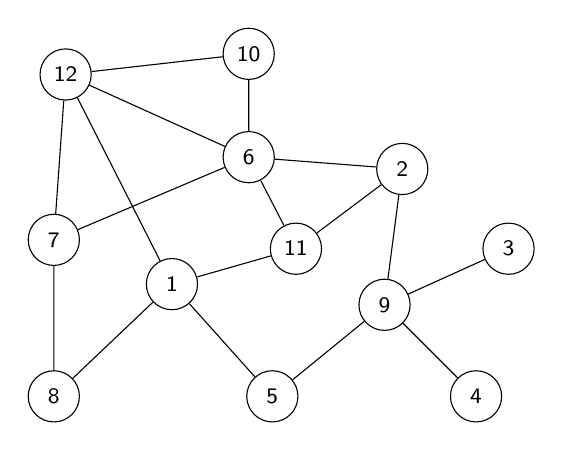
\begin{tikzpicture}[x=0.75cm,y=0.75cm,every node/.style={circle,draw,minimum size=6.5mm,inner sep=0pt,font=\sffamily\footnotesize}]
\node (12) at (1.3,-1.3) {12}; \node (10) at (4.4,-0.95) {10}; \node (6) at (4.4,-2.7) {6};
\node (2) at (7.0,-2.9) {2}; \node (7) at (1.1,-4.1) {7}; \node (11) at (5.2,-4.25) {11};
\node (3) at (8.8,-4.25) {3}; \node (1) at (3.1,-4.85) {1}; \node (9) at (6.7,-5.2) {9};
\node (8) at (1.1,-6.75) {8}; \node (5) at (4.8,-6.75) {5}; \node (4) at (8.25,-6.75) {4};
\draw (12)--(10) (12)--(6) (12)--(7) (12)--(1) (10)--(6) (6)--(2) (6)--(7) (6)--(11) (2)--(11) (2)--(9)
      (11)--(1) (7)--(8) (1)--(8) (1)--(5) (9)--(3) (9)--(5) (9)--(4);
\end{tikzpicture}
\end{center}
a.~1, 12, 10, 6, 11, 2, 9, 5, 4, 3, 7, 8\\
b.~1, 5, 8, 11, 12, 9, 7, 2, 6, 10, 3, 4\\
c.~1, 12, 11, 8, 5, 10, 7, 6, 2, 9, 4, 3\\
d.~1, 5, 9, 2, 6, 7, 8, 12, 10, 11, 3, 4

\item (3\%) What will we get after we heapify the integer array \{19, 5, 27, 3, 16, 11, 69, 18\} to a Max Heap in $O(n)$ time? Note that we use the bottom-up method.

a. \{69, 27, 19, 18, 16, 11, 5, 3\} \qquad b. \{69, 18, 27, 5, 16, 11, 19, 3\}\\
c. \{69, 18, 27, 16, 5, 11, 19, 3\} \qquad d. \{3, 5, 11, 16, 18, 19, 27, 69\}

\item (3\%) Please select the result after we add the integers \{89, 70, 52, 4, 25, 99, 59, 20, 79, 62, 44, 38\} sequentially to an AVL tree.
\begin{center}
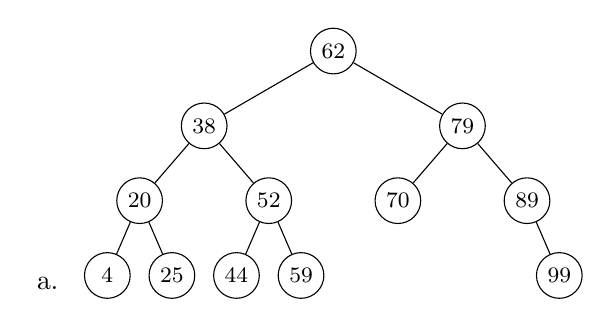
\begin{tikzpicture}[x=0.82cm,y=0.95cm,baseline=(current bounding box.south),tn/.style={circle,draw,minimum size=5.8mm,inner sep=0pt,font=\footnotesize}]
\node[tn] (n62) at (0.00,0.00) {62};
\node[tn] (n38) at (-2.00,-1.00) {38};
\node[tn] (n20) at (-3.00,-2.00) {20};
\node[tn] (n4) at (-3.50,-3.00) {4};
\node[tn] (n25) at (-2.50,-3.00) {25};
\node[tn] (n52) at (-1.00,-2.00) {52};
\node[tn] (n44) at (-1.50,-3.00) {44};
\node[tn] (n59) at (-0.50,-3.00) {59};
\node[tn] (n79) at (2.00,-1.00) {79};
\node[tn] (n70) at (1.00,-2.00) {70};
\node[tn] (n89) at (3.00,-2.00) {89};
\node[tn] (n99) at (3.50,-3.00) {99};
\draw (n62) -- (n38);
\draw (n38) -- (n20);
\draw (n20) -- (n4);
\draw (n20) -- (n25);
\draw (n38) -- (n52);
\draw (n52) -- (n44);
\draw (n52) -- (n59);
\draw (n62) -- (n79);
\draw (n79) -- (n70);
\draw (n79) -- (n89);
\draw (n89) -- (n99);
\node[anchor=south east] at ([xshift=-2mm]current bounding box.south west) {a.};
\end{tikzpicture}\hfill
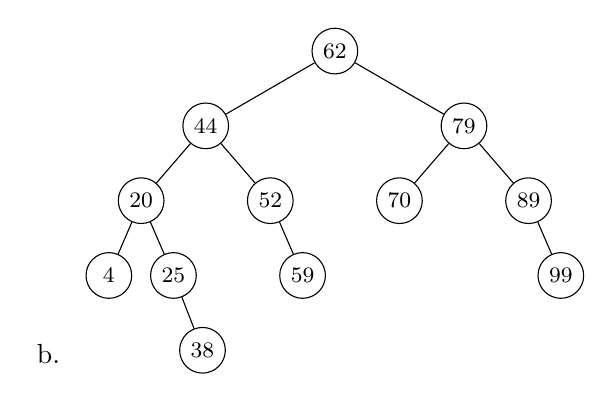
\begin{tikzpicture}[x=0.82cm,y=0.95cm,baseline=(current bounding box.south),tn/.style={circle,draw,minimum size=5.8mm,inner sep=0pt,font=\footnotesize}]
\node[tn] (n62) at (0.00,0.00) {62};
\node[tn] (n44) at (-2.00,-1.00) {44};
\node[tn] (n20) at (-3.00,-2.00) {20};
\node[tn] (n4) at (-3.50,-3.00) {4};
\node[tn] (n25) at (-2.50,-3.00) {25};
\node[tn] (n38) at (-2.05,-4.00) {38};
\node[tn] (n52) at (-1.00,-2.00) {52};
\node[tn] (n59) at (-0.50,-3.00) {59};
\node[tn] (n79) at (2.00,-1.00) {79};
\node[tn] (n70) at (1.00,-2.00) {70};
\node[tn] (n89) at (3.00,-2.00) {89};
\node[tn] (n99) at (3.50,-3.00) {99};
\draw (n62) -- (n44);
\draw (n44) -- (n20);
\draw (n20) -- (n4);
\draw (n20) -- (n25);
\draw (n25) -- (n38);
\draw (n44) -- (n52);
\draw (n52) -- (n59);
\draw (n62) -- (n79);
\draw (n79) -- (n70);
\draw (n79) -- (n89);
\draw (n89) -- (n99);
\node[anchor=south east] at ([xshift=-2mm]current bounding box.south west) {b.};
\end{tikzpicture}

\medskip
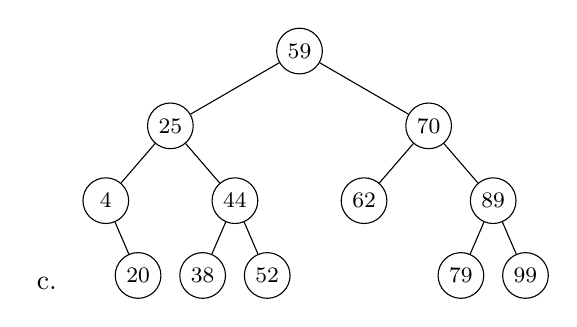
\begin{tikzpicture}[x=0.82cm,y=0.95cm,baseline=(current bounding box.south),tn/.style={circle,draw,minimum size=5.8mm,inner sep=0pt,font=\footnotesize}]
\node[tn] (n59) at (0.00,0.00) {59};
\node[tn] (n25) at (-2.00,-1.00) {25};
\node[tn] (n4) at (-3.00,-2.00) {4};
\node[tn] (n20) at (-2.50,-3.00) {20};
\node[tn] (n44) at (-1.00,-2.00) {44};
\node[tn] (n38) at (-1.50,-3.00) {38};
\node[tn] (n52) at (-0.50,-3.00) {52};
\node[tn] (n70) at (2.00,-1.00) {70};
\node[tn] (n62) at (1.00,-2.00) {62};
\node[tn] (n89) at (3.00,-2.00) {89};
\node[tn] (n79) at (2.50,-3.00) {79};
\node[tn] (n99) at (3.50,-3.00) {99};
\draw (n59) -- (n25);
\draw (n25) -- (n4);
\draw (n4) -- (n20);
\draw (n25) -- (n44);
\draw (n44) -- (n38);
\draw (n44) -- (n52);
\draw (n59) -- (n70);
\draw (n70) -- (n62);
\draw (n70) -- (n89);
\draw (n89) -- (n79);
\draw (n89) -- (n99);
\node[anchor=south east] at ([xshift=-2mm]current bounding box.south west) {c.};
\end{tikzpicture}\hfill
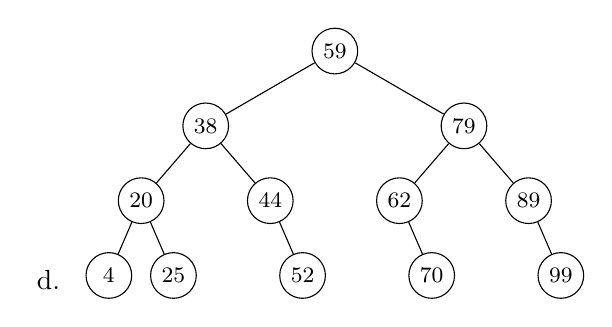
\begin{tikzpicture}[x=0.82cm,y=0.95cm,baseline=(current bounding box.south),tn/.style={circle,draw,minimum size=5.8mm,inner sep=0pt,font=\footnotesize}]
\node[tn] (n59) at (0.00,0.00) {59};
\node[tn] (n38) at (-2.00,-1.00) {38};
\node[tn] (n20) at (-3.00,-2.00) {20};
\node[tn] (n4) at (-3.50,-3.00) {4};
\node[tn] (n25) at (-2.50,-3.00) {25};
\node[tn] (n44) at (-1.00,-2.00) {44};
\node[tn] (n52) at (-0.50,-3.00) {52};
\node[tn] (n79) at (2.00,-1.00) {79};
\node[tn] (n62) at (1.00,-2.00) {62};
\node[tn] (n70) at (1.50,-3.00) {70};
\node[tn] (n89) at (3.00,-2.00) {89};
\node[tn] (n99) at (3.50,-3.00) {99};
\draw (n59) -- (n38);
\draw (n38) -- (n20);
\draw (n20) -- (n4);
\draw (n20) -- (n25);
\draw (n38) -- (n44);
\draw (n44) -- (n52);
\draw (n59) -- (n79);
\draw (n79) -- (n62);
\draw (n62) -- (n70);
\draw (n79) -- (n89);
\draw (n89) -- (n99);
\node[anchor=south east] at ([xshift=-2mm]current bounding box.south west) {d.};
\end{tikzpicture}
\end{center}

\item (3\%) Please select the correct number of distinct binary trees with 8 nodes.

a. 1430 \qquad b. 132 \qquad c. 429 \qquad d. 4862

\item (3\%) Please select the result after we add the integers \{50, 10, 80, 90, 70, 60, 65, 62\} sequentially to a red-black tree. Note that the following white and black circles represent the red and black nodes in red-black trees, respectively.
\begin{center}
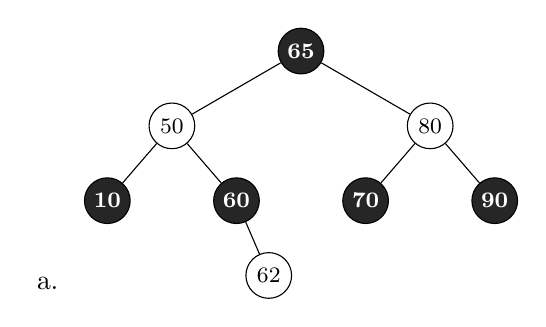
\begin{tikzpicture}[x=0.82cm,y=0.95cm,baseline=(current bounding box.south),
  rn/.style={circle,draw,minimum size=5.8mm,inner sep=0pt,font=\footnotesize},bn/.style={rn,fill=black!85,text=white,font=\footnotesize\bfseries}]
\node[bn] (n65) at (0.00,0.00) {65};
\node[rn] (n50) at (-2.00,-1.00) {50};
\node[bn] (n10) at (-3.00,-2.00) {10};
\node[bn] (n60) at (-1.00,-2.00) {60};
\node[rn] (n62) at (-0.50,-3.00) {62};
\node[rn] (n80) at (2.00,-1.00) {80};
\node[bn] (n70) at (1.00,-2.00) {70};
\node[bn] (n90) at (3.00,-2.00) {90};
\draw (n65) -- (n50);
\draw (n50) -- (n10);
\draw (n50) -- (n60);
\draw (n60) -- (n62);
\draw (n65) -- (n80);
\draw (n80) -- (n70);
\draw (n80) -- (n90);
\node[anchor=south east] at ([xshift=-2mm]current bounding box.south west) {a.};
\end{tikzpicture}\hfill
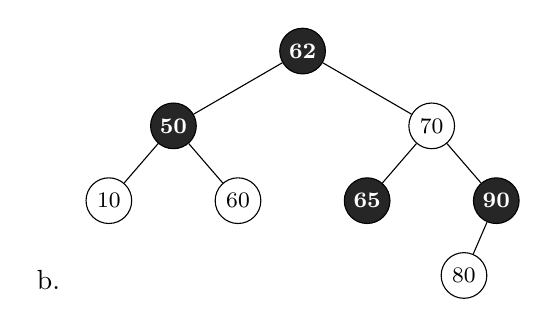
\begin{tikzpicture}[x=0.82cm,y=0.95cm,baseline=(current bounding box.south),
  rn/.style={circle,draw,minimum size=5.8mm,inner sep=0pt,font=\footnotesize},bn/.style={rn,fill=black!85,text=white,font=\footnotesize\bfseries}]
\node[bn] (n62) at (0.00,0.00) {62};
\node[bn] (n50) at (-2.00,-1.00) {50};
\node[rn] (n10) at (-3.00,-2.00) {10};
\node[rn] (n60) at (-1.00,-2.00) {60};
\node[rn] (n70) at (2.00,-1.00) {70};
\node[bn] (n65) at (1.00,-2.00) {65};
\node[bn] (n90) at (3.00,-2.00) {90};
\node[rn] (n80) at (2.50,-3.00) {80};
\draw (n62) -- (n50);
\draw (n50) -- (n10);
\draw (n50) -- (n60);
\draw (n62) -- (n70);
\draw (n70) -- (n65);
\draw (n70) -- (n90);
\draw (n90) -- (n80);
\node[anchor=south east] at ([xshift=-2mm]current bounding box.south west) {b.};
\end{tikzpicture}

\medskip
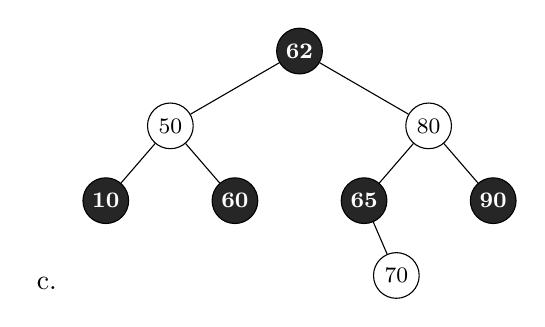
\begin{tikzpicture}[x=0.82cm,y=0.95cm,baseline=(current bounding box.south),
  rn/.style={circle,draw,minimum size=5.8mm,inner sep=0pt,font=\footnotesize},bn/.style={rn,fill=black!85,text=white,font=\footnotesize\bfseries}]
\node[bn] (n62) at (0.00,0.00) {62};
\node[rn] (n50) at (-2.00,-1.00) {50};
\node[bn] (n10) at (-3.00,-2.00) {10};
\node[bn] (n60) at (-1.00,-2.00) {60};
\node[rn] (n80) at (2.00,-1.00) {80};
\node[bn] (n65) at (1.00,-2.00) {65};
\node[rn] (n70) at (1.50,-3.00) {70};
\node[bn] (n90) at (3.00,-2.00) {90};
\draw (n62) -- (n50);
\draw (n50) -- (n10);
\draw (n50) -- (n60);
\draw (n62) -- (n80);
\draw (n80) -- (n65);
\draw (n65) -- (n70);
\draw (n80) -- (n90);
\node[anchor=south east] at ([xshift=-2mm]current bounding box.south west) {c.};
\end{tikzpicture}\hfill
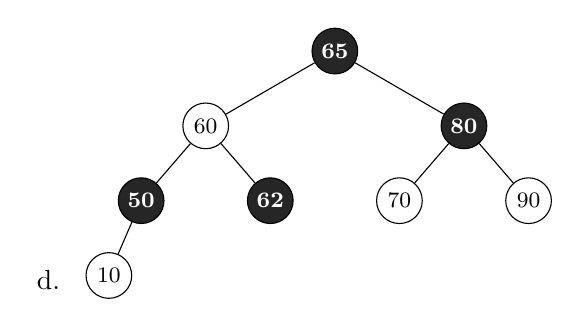
\begin{tikzpicture}[x=0.82cm,y=0.95cm,baseline=(current bounding box.south),
  rn/.style={circle,draw,minimum size=5.8mm,inner sep=0pt,font=\footnotesize},bn/.style={rn,fill=black!85,text=white,font=\footnotesize\bfseries}]
\node[bn] (n65) at (0.00,0.00) {65};
\node[rn] (n60) at (-2.00,-1.00) {60};
\node[bn] (n50) at (-3.00,-2.00) {50};
\node[rn] (n10) at (-3.50,-3.00) {10};
\node[bn] (n62) at (-1.00,-2.00) {62};
\node[bn] (n80) at (2.00,-1.00) {80};
\node[rn] (n70) at (1.00,-2.00) {70};
\node[rn] (n90) at (3.00,-2.00) {90};
\draw (n65) -- (n60);
\draw (n60) -- (n50);
\draw (n50) -- (n10);
\draw (n60) -- (n62);
\draw (n65) -- (n80);
\draw (n80) -- (n70);
\draw (n80) -- (n90);
\node[anchor=south east] at ([xshift=-2mm]current bounding box.south west) {d.};
\end{tikzpicture}
\end{center}
\end{enumerate}
\end{pastexam}

\begin{pastsoln}
答案：(1) d；(2) b；(3) c；(4) a；(5) a。

五個小題分屬資結書第~21~章（DFS）、第~8~章（建堆積）、第~10~章（AVL 樹、紅黑樹）、第~7~章（二元樹
個數）；AVL 樹和紅黑樹兩小題最吃重，放在第~10~章。

\textbf{(1) DFS：d。} 先列出每個點的鄰居（由小到大）：
\begin{center}
\small
\begin{tabular}{ll@{\qquad}ll@{\qquad}ll}
1 & 5, 8, 11, 12 & 5 & 1, 9 & 9 & 2, 3, 4, 5 \\
2 & 6, 9, 11 & 6 & 2, 7, 10, 11, 12 & 10 & 6, 12 \\
3 & 9 & 7 & 6, 8, 12 & 11 & 1, 2, 6 \\
4 & 9 & 8 & 1, 7 & 12 & 1, 6, 7, 10 \\
\end{tabular}
\end{center}
從 1 出發，每次走到編號最小的未拜訪鄰居，沒有就退回（資結書第~21.4~節）：
1 $\to$ 5 $\to$ 9 $\to$ 2 $\to$ 6 $\to$ 7 $\to$ 8（8 的鄰居 1、7 都拜訪過，退回 7）$\to$ 12（12 的鄰居
1、6、7 都拜訪過）$\to$ 10（10 的鄰居都拜訪過，一路退回 6）$\to$ 11（退回 2、再退回 9）$\to$ 3
$\to$ 4。 拜訪順序 1, 5, 9, 2, 6, 7, 8, 12, 10, 11, 3, 4，是 d。 a、c 一開始就走 12，但 1 的鄰居裡 5 最小；
b 的 1 之後是 5、8，但 5 的鄰居只有 1、9，下一個應該是 9。

\textbf{(2) 由下而上建最大堆積：b。} 照資結書虛擬碼~8.3，從最後一個內部節點（位置 $4$）往前，每個
位置做一次下沉。 陣列位置 $1$--$8$：
\begin{center}
\small
\begin{tabular}{>{\raggedright\arraybackslash}p{0.55\linewidth}l}
\toprule
步驟 & 陣列 \\
\midrule
開始 & 19, 5, 27, 3, 16, 11, 69, 18 \\
位置 4（3）：子節點 18 較大，交換 & 19, 5, 27, \textbf{18}, 16, 11, 69, \textbf{3} \\
位置 3（27）：子節點 11、69，69 較大，交換 & 19, 5, \textbf{69}, 18, 16, 11, \textbf{27}, 3 \\
位置 2（5）：子節點 18、16，18 較大，交換；5 再和子節點 3 比，不動 & 19, \textbf{18}, 69, \textbf{5}, 16, 11, 27, 3 \\
位置 1（19）：和 69 交換；19 再和子節點 11、27 比，和 27 交換 & \textbf{69}, 18, \textbf{27}, 5, 16, 11, \textbf{19}, 3 \\
\bottomrule
\end{tabular}
\end{center}
結果 $\{69, 18, 27, 5, 16, 11, 19, 3\}$，是 b。 a（由大到小排好）和 c 也都滿足最大堆積的性質，但不是由下而上建出來的結果：位置 2 的 5 下沉時
和 18 交換、停在位置 4，所以位置 4 是 5、位置 5 是 16，c 剛好相反。 d 是由小到大排好，根不是最大值，
不是最大堆積。

\textbf{(3) AVL 樹：c。} 依序插入，失衡時照資結書第~10.2.3~節的四種情形旋轉（括號裡是子樹，$-$ 表示
空）：
\begin{itemize}
\item 89、70、52：52 插在 70 的左邊，89 的平衡因子 $+2$，LL，在 89 右旋：70(52, 89)。
\item 4：70(52(4, $-$), 89)。 25：插在 4 的右邊，52 失衡，LR：先在 4 左旋、再在 52 右旋，得
70(25(4, 52), 89)。
\item 99、59、20、79 都直接插入，不失衡：70(25(4($-$, 20), 52($-$, 59)), 89(79, 99))。
\item 62：插在 59 的右邊，52 的平衡因子 $-2$，RR，在 52 左旋：
70(25(4($-$, 20), 59(52, 62)), 89(79, 99))。
\item 44：路徑 70 $\to$ 25 $\to$ 59 $\to$ 52，插在 52 的左邊。 70 的左子樹高 $3$、右子樹高 $1$，失衡；
44 在 70 的左子節點 25 的\textbf{右}子樹裡，LR：先在 25 左旋（59 上來），再在 70 右旋：
59(25(4($-$, 20), 52(44, $-$)), 70(62, 89(79, 99)))。
\item 38：路徑 59 $\to$ 25 $\to$ 52 $\to$ 44，插在 44 的左邊，52 的平衡因子 $+2$，LL，在 52 右旋：
59(25(4($-$, 20), 44(38, 52)), 70(62, 89(79, 99)))。
\end{itemize}
最後的樹：根 59；左子樹 25，其下 4（右子節點 20）和 44（子節點 38、52）；右子樹 70，其下 62 和
89（子節點 79、99），是 c。 a、b、d 都不是這個形狀：a、b 的根是 62，d 的 25 位置放了 38。

\textbf{(4) 8 個節點的二元樹個數：a。} $n$ 個節點、形狀不同的二元樹有 Catalan 數
$C_n = \frac{1}{n + 1}\binom{2n}{n}$ 棵（資結書定理~7.6）。
$C_8 = \frac{1}{9}\binom{16}{8} = \frac{12870}{9} = 1430$。 其他選項：$132 = C_6$、$429 = C_7$、
$4862 = C_9$。

\textbf{(5) 紅黑樹：a。} 照資結書虛擬碼~10.6 的插入修正（新節點是紅色；父節點是紅色時，看叔叔的
顏色）。 下面 R、B 表示紅、黑：
\begin{itemize}
\item 50 當根，塗黑。 10、80 插在根的兩邊，紅色，父節點黑，不用修正。
\item 90：插在 80 的右邊。 父 80 紅、叔叔 10 紅，情形 1：80、10 塗黑，50 塗紅；50 是根，再塗回黑。
\item 70：插在 80 的左邊，父 80 黑，不用修正。 樹：50B(10B, 80B(70R, 90R))。
\item 60：插在 70 的左邊。 父 70 紅、叔叔 90 紅，情形 1：70、90 塗黑，80 塗紅；80 的父 50 黑，結束。
樹：50B(10B, 80R(70B(60R, $-$), 90B))。
\item 65：插在 60 的右邊。 父 60 紅、叔叔（70 的右子節點）是空的，算黑；65 是右子節點、60 是左子節點，
情形 2：在 60 左旋，變成 65 為 70 的左子節點、60 為 65 的左子節點；接著情形 3：65 塗黑、70 塗紅、
在 70 右旋。 樹：50B(10B, 80R(65B(60R, 70R), 90B))。
\item 62：插在 60 的右邊。 父 60 紅、叔叔 70 紅，情形 1：60、70 塗黑，65 塗紅，往上看 65。 65 的父 80
紅、叔叔 10 黑；65 是左子節點、80 是右子節點，情形 2：在 80 右旋（65 上來，80 變成 65 的右子節點），
接著情形 3：65 塗黑、50 塗紅、在 50 左旋。
\end{itemize}
最後的樹：根 65（黑）；左子節點 50（紅），其子節點 10（黑）、60（黑），60 的右子節點 62（紅）；右子節點
80（紅），其子節點 70（黑）、90（黑）。 這就是 a。 檢查：沒有紅節點有紅子節點，每條從根到空指標
的路徑都經過 $2$ 個黑節點（含根，不算空節點）。
\end{pastsoln}
